% $Id: admb-dll.tex 204 2009-04-20 01:59:36Z jsibert $
%
% Author: David Fournier
% Copyright (c) 2008 Regents of the University of California
%

For performance reasons, many nonlinear modeling routines for packages
such as Splus or Gauss, or spreadsheets such as Excel,
are written in other languages, such as C or \textsc{fortran}, and
compiled as \textsc{dll}s or shared libraries. Due to 
\ADM's support for nonlinear statistical modeling, it
is generally much faster and easier to produce the code for
a nonlinear statistical model with \textsc{admb} rather than C or \textsc{fortran}.
This code can then be put into a shared library (\textsc{dll}) and called
from Splus as though it were a part of the language. 

This section focuses on creating \textsc{dll}s for Splus Version~4 Release~3, Gauss
under Windows 95/NT,
or for the R programming environment under Windows 95/NT or Linux. 
The construction can be easily modified to produce \textsc{dll}s, which can be
used by other programs, such as Visual Basic, or spreadsheets like Excel.

There are two example programs: a very 
simple example to illustrate the ideas,
and a program to estimate the parameters from a mixture of two bivariate
normal distributions.
 
We begin with the simple example. We
wish to minimize the function $f$ given by
$$ f=(x_1-1.0)^2+\sum_{i=1}^{n-1}(x_{i+1}-x_i)^2$$
with respect to the $n$-dimensional vector $x$. The
starting values are $x=(0,0,\ldots,0)$.
   
While this is a quadratic function that can be solved by special methods,
we do not use this special structure, because we want to illustrate
the technique on general nonlinear models. 

There are three modifications to a stand-alone \ADM\ program
that must be made to produce a~\textsc{dll}.
\begin{enumerate}

\item The command line option \texttt{-dll} is given to the
\texttt{tpl2cpp} program, which translates the template file into a
\cplus\ file. For Gauss, replace the \texttt{-dll} option with
the \texttt{-gausdll} option.
\XX{\fontindexentry{tt}{-dll}}{command line option}
\XX{command line arguments}{\fontindexentry{tt}{-dll}}

\item The user must decide what data and parameter
objects are to be passed to, or returned from, the \textsc{dll},
and modify the \textsc{tpl} file accordingly.

\item The interface code must be written in the
calling language. 
\end{enumerate}

Objects that are to be passed into, or returned from, the
\textsc{dll} are identified by putting the prefix \texttt{dll\_}
before their declarations.

In this example, the number of independent variables
is passed from the calling program to the \textsc{dll}.
Thus, \texttt{init\_int nvar} is modified to 
\texttt{dll\_init\_int nvar}. The calling program
expects to get the minimum value \texttt{freturn}
and the minimizing values
of the {init\_vector x} returned to it, so they are declared to be
of type \texttt{dll\_number} and \texttt{dll\_init\_vector}.
\begin{lstlisting}
DATA_SECTION
  dll_int nvar
PARAMETER_SECTION
  dll_init_vector x(1,nvar)
  dll_number freturn
  objective_function_value f
PROCEDURE_SECTION
  f=square(x(1)-1.0);
  for (int i=1;i<nvar;i++)
  {
    f+=square(x(i+1)-x(i));
  }
  freturn=f;
\end{lstlisting}


\XX{\fontindexentry{sc}{dll}}{commands for producing}
\section{Compiling the code to produce a \textsc{dll}}

The exact form of the commands used to produce a \textsc{dll}, or shared library,
depend on the compiler used and the operating system.

Assuming that the template file is named \texttt{xxxx.tpl|}
for NT/9?, then using the gcc2.95-mingw32 compiler, the 
commands are 
\begin{lstlisting}
tpl2cpp -dll  %1

 C++ -fpermissive -O3 -c -DBUILDING_DLL=1 -D__GNUDOS__ -I. i
  -If:/admodel/include   -o %1.o %1.cpp

dllwrap -def %1.def --implib lib%1.a --driver-name \cplus\ -o %1.dll  %1.o 
   -Lf:/admodel/lib -ladmod -ladt -lado -lm 
\end{lstlisting}
where the symbol \texttt{\%1} (this is a batch file argument, which would
be \texttt{\$1} for Linux) should be replaced by \texttt{xxxx}.

Of course, you don't want to type all this every time, so the commands
should be replaced in a \texttt{.bat} file,
such as \texttt{makedll.bat}.
Then, to compile the \textsc{tpl} into a \textsc{dll}, it is only necessary to type
\begin{lstlisting}
  makeadll xxxx
\end{lstlisting}
where \texttt{xxxx.tpl} is the template file.
For debugging purposes, you may find that you want to edit the
\texttt{.cpp} file, so you will not want to run \texttt{tpl2cpp}
every time. In that case, the first line should be removed from
the \texttt{.bat} file.

To call the \textsc{dll} from Splus, the \texttt{dll.load} function is used to
load the library. 
\begin{smallcode}
dll.load("simpdll.dll",symbol="simpdll")
n<-100
x<-rep(0,n)
freturn<-0
ans<-.C("simpdll",as.integer(n),x = as.double(x),as.double(f)," -sp -crit 1.e-8 -nohess")
\end{smallcode}
The final parameter, \texttt{-sp -crit 1.e-8 -nohess}, is a string that serves the same function as command
line options in AD Model Builder programs. 
The \texttt{-sp} option tells the \textsc{dll} that it is being run from Splus, so 
it can print into the Splus command window. The \texttt{-crit} option sets the
convergence criterion for the magnitude of the components of the
gradient, and the \texttt{-nohess} option suppresses the calculation of the 
Hessian at the minimum. It must be present, although it can be blank.

It is necessary for Splus to find the \textsc{dll}. If it has trouble doing so, a full
path name can be used as in:
\begin{lstlisting}
  dll.load("c://mydlls//simpdll.dll",symbol="simpdll")
\end{lstlisting}


\section{The Splus objects}

At present, the objects for communication
with Splus that can be put in the \DS\ of the \textsc{tpl} file are
\begin{lstlisting}
dll_init_int
dll_iinit_number
dll_iinit_vector
dll_init_matrix
dll_int
dll_number
dll_vector
dll_matrix
\end{lstlisting}
while in the \texttt{PARAMETER\_SECTION}, they are
\begin{lstlisting}
dll_init_number
dll_init_bounded_number
dll_init_vector
dll_init_bounded_vector
dll_init_matrix
dll_number
dll_vector
dll_matrix
\end{lstlisting}
These objects act the same as the corresponding AD Model Builder objects
without the \texttt{dll\_} prefix. For initial parameters, the difference is that
they are assumed to get their initial values from Splus.

Note that by default, Splus stores elements of a matrix by columns, that
is, contiguous areas of memory run down the columns. AD Model Builder stores
its elements by rows, so that when a matrix objects is passed to it from
Splus, it expects the object to be stored by column and does a transpose
operation on it. At the conclusion of the AD Model Builder program,
the object is passed back to Splus via the inverse operation. This
process should be transparent to the user. 

Gauss, on the other hand, stores a matrix by rows. 
In addition, Gauss passes a string as a \texttt{char *} rather than the
\texttt{char **} employed by Splus.
Using the \texttt{-gaussdll}
option ensures that Gauss matrices and strings will be handled properly.
\XX{\fontindexentry{tt}{-gaussdll}}{command line option}
\XX{command line arguments}{\fontindexentry{tt}{-gaussdll}}


\section{Debugging the \textsc{dll}s}
\XX{\fontindexentry{sc}{dll}}{debugging}

Before you compile your program as a \textsc{dll}, it is easiest if you
first compile it as a stand-alone application and debug it.
Then you can simply put the \texttt{dll\_} prefix before
those objects you wish to have passed to and from
the calling program.
Also is inconvenient to debug the \textsc{dll}s from Splus directly.
Errors in the code usually cause Splus to crash. 
Also, printing results to the screen from a \textsc{dll} can
be problematic if the calling program does not
provide for it. To alleviate this
problem, it is possible to call the function in the \textsc{dll}
from a C or \cplus\ routine. This enables the use of symbolic debuggers, etc.,
to debug the code, and enables screen I/O. 
Here is C code that can load the \textsc{dll} and call the function:
\begin{lstlisting}
#include <stdio.h>
#include <windows.h>

typedef __declspec(dllexport) void _export (*MYPROC)(int *_nvar,
  double *_x, 
  double *_freturn,
  char ** sp_options);

VOID main(int argc,char * argv[])
{
  HINSTANCE h;
  MYPROC p;
  /* Now invent the objects we need to pass to the DLL */
  int nvar=50;
  double x[50];
  double freturn;
  char * str;
  int i;
  char * str = " -nox -crit 1.e-7 ";
  h=LoadLibrary("simpdll"); /* load the DLL */
  if (h)
  {
    printf("loaded simdll.dll successfully\n");
    /* get pointer to the function */  
    p=(MYPROC) GetProcAddress(h,"_simpdll");
    if (p)
    {
      freturn=0.0;
      for (i=0;i<nvar;i++)
        x[i]=0.0;
      p(&nvar,x,&freturn,&str);
      
      printf("function value = %lf\n",&freturn);
      for (i=0;i<nvar;i++)
        printf("x[%d]= %lf\n",i,x[i]);
      
    }
    else
      printf("Can't find function simdll in DLL\n");
  }
  else
   printf("Can't load simdll.dll\n");
}
\end{lstlisting}
This code can be compiled with the command
\begin{lstlisting}
  gcc -otestsim.exe testsim.c
\end{lstlisting}
which will produce the program
\texttt{testsim.exe}. Running this program will 
load the \textsc{dll}, find the function in it, and call it.
At the end, it will report the results obtained.


\section{Understanding what is being passed to the \textsc{dll}}

The most difficult part of calling a \cplus\ \textsc{dll} from some other
type of application is understanding the correct formalism 
for passing different objects between the two.
For example, a string in Visual Basic
may be a very different object from the simple \texttt{char *}
(pointer to char) of the C and \cplus\ languages. If you get it wrong,
then the program will usually crash when the code in the \textsc{dll}
tries to access the object.  The easiest way to debug this is
to have the \textsc{dll} code print out the values of the passed
objects. (However, keep in mind that simply trying to access the
values for printing may cause the program to crash.)

Consider the \cplus\ for the example \textsc{tpl} code given above:
\begin{lstlisting}
#include <admodel.h>

#include <simpdll.htp>

model_data::model_data(splus_args& ad_spa)
{
  nvar.allocate(ad_spa.nvar,"nvar");
}

model_parameters::model_parameters(int sz,
  int argc, 
  char * argv[], 
  splus_args& ad_spa) : 
 ad_comm(argc,argv), model_data(ad_spa) , function_minimizer(sz)
{
  initializationfunction();
  x.allocate(ad_spa.x,1,nvar,"x");
  freturn.allocate(ad_spa.freturn,"freturn");
  f.allocate("f");
}

void model_parameters::userfunction(void)
{
  f=square(x(1)-1.0);
  for (int i=1;i<nvar;i++)
  {
    f+=square(x(i+1)-x(i));
  }
  freturn=f;
}

void model_parameters::preliminary_calculations(void){}

model_data::~model_data()
{}

model_parameters::~model_parameters()
{}

void model_parameters::report(void){}

void model_parameters::final_calcs(void){}

void model_parameters::set_runtime(void){}

#ifdef _BORLANDC_
  extern unsigned _stklen=10000U;
#endif


#ifdef __ZTC__
  extern unsigned int _stack=10000U;
#endif

  long int arrmblsize=0;
extern "C" {

#if !defined(__delcspec)
#  define __declspec(x)
#endif

#if !defined(__BORLANDC__)
#  define _export
#endif

__declspec(dllexport) void _export simpdll(int *_nvar,
  double *_x,
  double *_freturn,
  char ** sp_options)
{
  int argc=1;
  try {
    char **argv=parse_sp_options("simpdll",argc,*sp_options);
    do_dll_housekeeping(argc,argv);
    splus_args ad_spa(_nvar,_x,_freturn);
    gradient_structure::set_NO_DERIVATIVES();
    gradient_structure::set_YES_SAVE_VARIABLES_VALUES();
  #if defined(__GNUDOS__) || defined(DOS386) || defined(__DPMI32__)  || \
     defined(__MSVC32__)
      if (!arrmblsize) arrmblsize=150000;
  #else
      if (!arrmblsize) arrmblsize=25000;
  #endif
    model_parameters mp(arrmblsize,argc,argv,ad_spa);
    mp.iprint=10;
    mp.preliminary_calculations();
    mp.computations(argc,argv);
    cleanup_argv(argc,&argv);
    ad_make_code_reentrant();
  }
  catch (spdll_exception spe){ 
    if (ad_printf && spe.e) (*ad_printf) ("abnormal exit from newtest\n");
  }
}
}
\end{lstlisting}
For now, we are only interested in the 
part of the code after the beginning of the function
\begin{lstlisting}
__declspec(dllexport) void _export simpdll(int *_nvar,
  double *_x,
  double *_freturn,
  char ** sp_options)
{
  int argc=1;
  try {
  .....
\end{lstlisting}
Modify this code to:
\begin{lstlisting}
__declspec(dllexport) void _export simpdll(int *_nvar,
  double *_x,
  double *_freturn,
  char ** sp_options)
{
  cout << " nvar = " << *_nvar << endl;
  return; 
  int argc=1;
  try {
   .....
\end{lstlisting}
If everything is OK, this will simply print out the value of \texttt{nvar}
and return to the calling program.
Then the value of \texttt{x} can be printed out as well, with code like:
\begin{lstlisting}
__declspec(dllexport) void _export simpdll(int *_nvar,
  double *_x,
  double *_freturn,
  char ** sp_options)
{
  cout << " nvar = " << *_nvar << endl;
  cout << " x = " << endl;
  for (int i=0;i<*_nvar;i++)
    cout << _x[i] << endl;
  cout << " freturn = " << *_freturn << endl;
  cout << " sp_options = " << *sp_options << endl;
  return; 
  int argc=1;
  try {
   .....
\end{lstlisting}
If you don't have access to the screen, the above code can be modified to print to a file.
\begin{lstlisting}
__declspec(dllexport) void _export simpdll(int *_nvar,
  double *_x,
  double *_freturn,
  char ** sp_options)
{
  ofstream ofs("logfile");
  ofs << " nvar = " << *_nvar << endl;
  ofs << " x = " << endl;
  for (int i=0;i<*_nvar;i++)
    ofs << _x[i] << endl;
  ofs << " freturn = " << *_freturn << endl;
  ofs << " sp_options = " << *sp_options << endl;
  return; 
  int argc=1;
  try {
   .....
\end{lstlisting}
After running the program, you should find the values of the 
objects printed into a file named \texttt{logfile}.

Splus passes objects to the \textsc{dll} by address, that is, it
finds the address in memory of the object and passes that value.
So the integer \texttt{nvar} is not passed itself, but the address is. In
C or \cplus, you get the address of an object with the \texttt{\&}
operator.  Given the address of an object, you access the 
object with the \texttt{*} operator. In the above code,
\texttt{\_nvar} is the address of an integer passed by 
the calling program to the \textsc{dll} and \texttt{*\_nvar}
accesses the object. So, the line of code
\begin{lstlisting}
  *_nvar=5;
\end{lstlisting}
will set the values of the integer to 5 back in the calling 
program.
When Splus passes a vector object, it passes the address of the
first element in the vector. So, if the vector is a vector of
double precision numbers (an object of type \texttt{double} in C),
it will pass a pointer to \texttt{double}. So in the above code,
\texttt{\_x} is the address of the first element of the vector
and \texttt{*\_x} is the first element, so
\begin{lstlisting}
  *_x=12.55;
\end{lstlisting}
will set the first element in the vector equal to \texttt{12.55}.
To access other  elements of the vector, use the \texttt{[]} operators.
\begin{lstlisting}
x[0]=12.55;  // same as *_x=12.55
x[4]=-2.5;  // sets the 5 element equal to -2.5
\end{lstlisting}


\section{Passing strings from Splus to a \textsc{dll}}

A string in C is a pointer to an array of elements of type \texttt{char}.
It might be logical to conclude that Splus would pass the
address of the first element of the array. This is not
the case.  Splus passes the address of the object pointing to the 
first element of the array (a \texttt{char **} in C).
So in the above code, if you want to print the second element of the
string, point \texttt{sp\_options} to the standard output
device:
\begin{lstlisting}
  cout << (*sp_options)[1] << endl; // print the second element of the string
\end{lstlisting}
You must use the parentheses, because the \texttt{[]} operation has
higher precedence than does the \texttt{*}~operation.


\section{A mixture of two bivariate normal distributions}

This is a more complicated example.
Let $x_i$ be a collection of 2-dimensional vectors drawn  
at random from a mixture of two bivariate normal distributions with
means $\mu_i$ and covariance matrices $\Sigma_i$.
The data to be analyzed are shown here. They consist of 500
points from the mixture, with 25\% in one component and 75\% in the other
component. Both samples have positively correlated components, so
they both lie near the line $y=x$.
This makes them difficult to separate.
The means used for the simulations were
\begin{lstlisting}
  (0,0)     (1,0)
\end{lstlisting}
while the covariance matrices used for the simulation were
\begin{lstlisting}
1.77778 4.74074     1.77778 2.37037
4.74074 14.4198     2.37037 4.93827
\end{lstlisting}
The estimates for these parameters obtained by the model were
\begin{lstlisting}
(0.026,0.059)   (1.266,0.287)

1.42409 3.86336    1.66321 2.34985
3.86336 12.2286    2.34985 4.94363
\end{lstlisting}

The estimated proportions were
\begin{lstlisting}
    0.343  0.657
\end{lstlisting}
See Figure~\ref{fig:estimatedprop}.
\begin{figure}[h]
  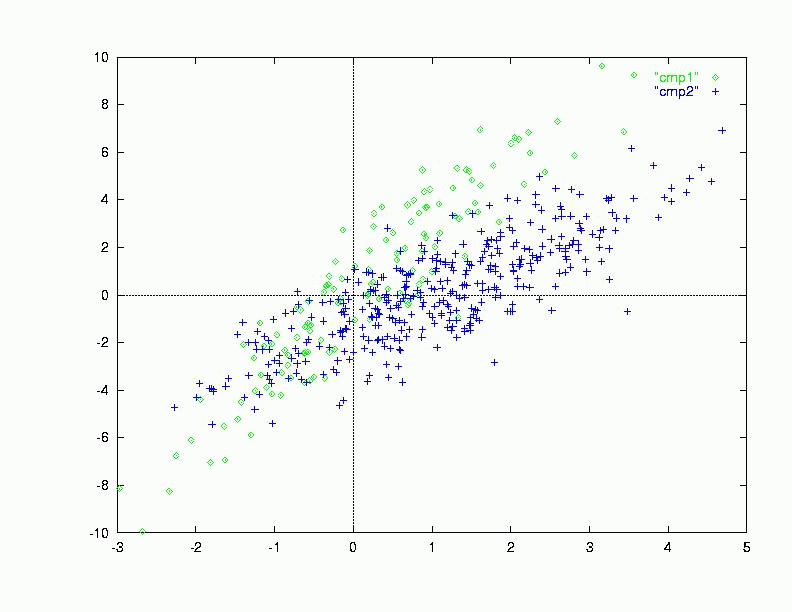
\includegraphics[height=4.5in, width=\textwidth]{datax.png}
  \emptycaption
  \label{fig:estimatedprop}
\end{figure}

The minimization is carried out in three phases. For the first phase, only
the proportions of the mixture are estimated, with the parameters that
determine the covariance matrices and the means held fixed. For the second
phase, the covariance matrices are estimated as well, with the means held fixed.
For the third and final phase, all the parameters are estimated.
The idea is that the user should start with some good estimates for
the means.  Of course, the model could be run several times with different
initial estimates and if different solutions are obtained, then the
one with the best fit would be chosen.

The initial values used for the means and standard deviations were
\begin{lstlisting}
(-1,0)   (2,0)

1  0     1  0
0  1     0  1
\end{lstlisting}
The initial values used for the proportions were
\begin{lstlisting}
    0.5      0.5
\end{lstlisting}
The log-likelihood  function for the sample is
 \begin{align}
  \nonumber \sum_{i=1}^n \log \Big\{&\,p_1|\Sigma_1|^{-1/2}\exp\big(\kern-.1em -0.5(x_i-\mu_1)^{\prime}\,
  \Sigma_1^{-1}(x_i-\mu_1)\big) \\
   &+p_2|\Sigma_2|^{-1/2}\exp\big(\kern-.1em -0.5(x_i-\mu_2)^{\prime}\,
  \Sigma_2^{-1}(x_i-\mu_2)\big) \Big\}
 \end{align}
The main technical difficulty in maximizing the log-likelihood
function is parameterizing the covariance matrices in such a way
that they will be positive definite. This is done by employing a
``positivized'' Choleksi decomposition.
$\Sigma_i$ as $\Sigma_i=C_iC_i^{\prime}+\lambda I$, where
$C_i$ is a lower triangular matrix, $\lambda>0$ is a ``small''
positive number, and $I$ is the identity matrix. 
The proportions in the mixture are parameterized by a bounded vector
of parameters that is normalized so that the components will sum to~1.
The code for the example follows:
\begin{lstlisting}
DATA_SECTION
  dll_int nobs
  dll_matrix obs(1,nobs,1,2) 
PARAMETER_SECTION
  dll_init_bounded_vector pcoff(1,2,.02,1.1);  
  dll_init_bounded_vector C1(1,3,-10.0,10.0,2)
  dll_init_bounded_vector C2(1,3,-10.0,10.0,2)
  dll_init_vector mu1(1,2,3)
  dll_init_vector mu2(1,2,3)
  dll_matrix S1(1,2,1,2)
  dll_matrix S2(1,2,1,2)
  dll_vector p(1,2)
  objective_function_value f
PROCEDURE_SECTION
  dvariable psum=sum(pcoff);
  f+=100.*square(log(psum+1.e-20));
  p=pcoff/(psum+1.e-20);  // so p's satisfy constraints
  dvar_matrix tmp1(1,2,1,2);
  dvar_matrix tmp2(1,2,1,2);
  tmp1.initialize();
  tmp2.initialize();
  int ii=1;
  int i=0;
  for (i=1;i<=2;i++) {   // fill lower triangle
    for (int j=1;j<=i;j++) { 
      tmp1(i,j)=C1(ii);
      tmp2(i,j)=C2(ii);
      ii++;
    }
  }
  S1=tmp1*trans(tmp1); // form S1 S2 from Choleski decomp.
  S2=tmp2*trans(tmp2);
  for (i=1;i<=2;i++) {  // to make positive definite
    S1(i,i)+=0.1; 
    S2(i,i)+=0.1;
  }
  dvariable det1=sqrt(det(S1));
  dvariable det2=sqrt(det(S2));
  dvar_matrix S1inv=inv(S1);
  dvar_matrix S2inv=inv(S2);
  for (i=1;i<=nobs;i++) // add up minus log-likelihood
  {
    // add the 1.e-10 to avoid log(0) and for robustness
    f-= log(1.e-10+p(1)/det1*exp(-.5*(obs(i)-mu1)*S1inv*(obs(i)-mu1))
       +p(2)/det2*exp(-.5*(obs(i)-mu2)*S2inv*(obs(i)-mu2)));
  }  
RUNTIME_SECTION
  maximum_function_evaluations 50,100,10000
REPORT_SECTION
  report << "First mean = " << endl << mu1 << endl;
  report << "First covariance matrix = " << endl<< S1 << endl;
  report << "Second mean = " << endl << mu2 << endl;
  report << "Second covariance matrix = " << endl << S2 << endl;
\end{lstlisting}

This example can be run by using the following Splus source code:
\begin{lstlisting}
 nobs<-scan("bimix.dat",n=1)
 x<-matrix(scan("bimix.dat",skip=1),nrow=nobs,ncol=2,byrow=TRUE)
 pcoff<-rep(.5,2)
 C1<-rep(1,3)
 C2<-rep(1,3)
 C1[2]<-0
 C2[2]<-0
 p<-rep(0,2)
 mu1<-rep(0,2)
 mu1[1]<--1
 mu2<-rep(0,2)
 mu2[1]<-2
 S1<-matrix(0,nrow=2,ncol=2)
 S2<-matrix(0,nrow=2,ncol=2)
 dll.load("bimix.dll",symbol="bimix")
 ans<-.C("bimix",nobs=as.integer(nobs),as.double(x),pcoff=as.double(pcoff),
   C1=as.double(C1),C2=as.double(C2),mu1=as.double(mu1),mu2=as.double(mu2),
   S1=as.double(S1),S2=as.double(S2),p=as.double(p)," -sp -nohess ") 
 dll.unload("bimix.dll")
 S1<-matrix(ans\$S1,nrow=2)  
 S2<-matrix(ans\$S2,nrow=2)  
 mu1<-ans\$mu1
 mu2<-ans\$mu2
 p<-ans\$p
 print ("Estimated proportions")
 print(p)
 print ("Estimated mean for component 1")
 print(mu1)
 print ("Estimated mean for component 2")
 print(mu2)
 print ("Estimated covariance matrix for component 1")
 print(S1)
 print ("Estimated covariance matrix for component 2")
 print(S2)
\end{lstlisting}
This code  only works under NT/95 for Version 4 Release~3.
Assuming that you have put the code where Splus can find it, you can
run the example from Splus by typing
\begin{lstlisting}
  source("bimix.spl")
\end{lstlisting}
There is also a file, \texttt{bimix.r}, which will run the program under~R.
However, at present for Windows, the R version will not print out any
intermediate results.  So, be patient and the final estimates will appear
when the minimization has converged.
After the program executes, the parameter estimates can be found in
the Splus variables \texttt{p}, \texttt{mu1}, \texttt{mu2}, \texttt{S1}, and~\texttt{S2}.


\section{Interpretation of the parameter estimates}

If the user desires, they can remove the \texttt{-nohess} option and have
the program compute estimates 
of the variances of the parameter estimates. %xx was nonsense.
\begin{lstlisting}
 index   name   value      std dev   
    1   pcoff  3.5511e-01  1.5693e+00
    2   pcoff  6.7911e-01  2.9777e+00
    3   C1     1.1507e+00  7.9990e-02
    4   C1     3.3574e+00  2.8240e-01
    5   C1     9.2537e-01  1.7504e-01
    6   C2     1.2503e+00  7.7426e-02
    7   C2     1.8795e+00  1.2641e-01
    8   C2     1.1451e+00  8.3415e-02
    9   mu     2.6366e-02  1.2791e-01
   10   mu     5.9418e-02  3.4832e-01
   11   mu     1.2627e+00  1.4717e-01
   12   mu     2.8665e-01  1.7818e-01
   13   p      3.4336e-01  6.7238e-02
   14   p      6.5664e-01  6.7238e-02
\end{lstlisting}

The program also reports the correlation matrix
\begin{tinycode}

 index   name    value     std dev     1     2      3      4      5      6      7      8      9     10     11     12     13     14 
     1   pcoff  3.551e-01 1.569e+00  1.000
    2   pcoff  6.791e-01 2.977e+00  0.997  1.000
    3   C1     1.150e+00 7.999e-02 -0.039 -0.021  1.000
    4   C1     3.357e+00 2.824e-01 -0.094 -0.052  0.736  1.000
    5   C1     9.253e-01 1.750e-01  0.067  0.036  0.031 -0.394  1.000
    6   C2     1.250e+00 7.742e-02 -0.071 -0.039  0.156  0.266 -0.070  1.000
    7   C2     1.879e+00 1.264e-01 -0.016 -0.009 -0.066 -0.046 -0.087  0.613  1.000
    8   C2     1.145e+00 8.341e-02 -0.072 -0.039  0.031  0.343 -0.308  0.138 -0.116  1.000
    9   mu     2.636e-02 1.279e-01 -0.000 -0.000  0.147 -0.054  0.285  0.349  0.163 -0.212  1.000
   10   mu     5.941e-02 3.483e-01 -0.045 -0.024  0.198  0.160 -0.012  0.411  0.245 -0.066  0.861  1.000
   11   mu     1.262e+00 1.471e-01  0.115  0.063 -0.295 -0.521  0.257 -0.572 -0.170 -0.322 -0.225 -0.421  1.000
   12   mu     2.866e-01 1.781e-01  0.063  0.034 -0.237 -0.247  0.071 -0.482 -0.265  0.003 -0.363 -0.460  0.803  1.000
   13   p      3.433e-01 6.723e-02  0.148  0.081 -0.266 -0.636  0.450 -0.482 -0.111 -0.487 -0.001 -0.302  0.773  0.426  1.000
   14   p      6.566e-01 6.723e-02 -0.148 -0.081  0.266  0.636 -0.450  0.482  0.111  0.487  0.001  0.302 -0.773 -0.426 -1.000  1.000
\end{tinycode}
